\section{USING THE TEMPLATE}

Use this sample document as your LaTeX source file to create your document. Save this file as {\bf root.tex}. You have to make sure to use the cls file that came with this distribution. If you use a different style file, you cannot expect to get required margins. Note also that when you are creating your out PDF file, the source file is only part of the equation. {\it Your \TeX\ $\rightarrow$ PDF filter determines the output file size. Even if you make all the specifications to output a letter file in the source - if your filter is set to produce A4, you will only get A4 output. }

It is impossible to account for all possible situation, one would encounter using \TeX. If you are using multiple \TeX\ files you must make sure that the ``MAIN`` source file is called root.tex - this is particularly important if your conference is using PaperPlaza's built in \TeX\ to PDF conversion tool.

\subsection{Headings, etc}

Text heads organize the topics on a relational, hierarchical basis. For example, the paper title is the primary text head because all subsequent material relates and elaborates on this one topic. If there are two or more sub-topics, the next level head (uppercase Roman numerals) should be used and, conversely, if there are not at least two sub-topics, then no subheads should be introduced. Styles named Heading 1, Heading 2, Heading 3, and Heading 4 are prescribed.

\subsection{Figures and Tables}

Positioning Figures and Tables: Place figures and tables at the top and bottom of columns. Avoid placing them in the middle of columns. Large figures and tables may span across both columns. Figure captions should be below the figures; table heads should appear above the tables. Insert figures and tables after they are cited in the text. Use the abbreviation Fig. 1, even at the beginning of a sentence.

\begin{table}[h]
  \caption{An Example of a Table}
  \label{table:example}
  \begin{center}
    \begin{tabular}{|c||c|}
      \hline
      One & Two\\
      \hline
      Three & Four\\
      \hline
    \end{tabular}
  \end{center}
\end{table}


\begin{figure}[thpb]
  \centering
  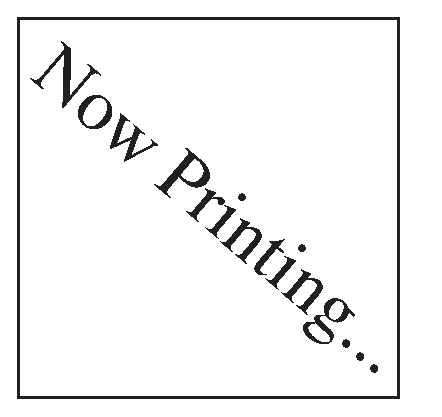
\includegraphics[width=\columnwidth]{nowprinting.eps}
  \caption{Inductance of oscillation winding on amorphous
    magnetic core versus DC bias magnetic field}
  \label{figure:label}
\end{figure}


Figure Labels: Use 8 point Times New Roman for Figure labels. Use words rather than symbols or abbreviations when writing Figure axis labels to avoid confusing the reader. As an example, write the quantity Magnetization, or Magnetization, M, not just M. If including units in the label, present them within parentheses. Do not label axes only with units. In the example, write Magnetization (A/m) or Magnetization {A[m(1)]}, not just A/m. Do not label axes with a ratio of quantities and units. For example, write Temperature (K), not Temperature/K.

